\documentclass{beamer}
\usetheme{Pittsburgh}
\beamertemplatenavigationsymbolsempty


\usepackage{amsmath}
\usepackage{amssymb}
\usepackage{bm} % For bold math symbols
\usepackage{graphicx}
\usepackage{tikz}



\usepackage{subfig} % Changed from subfigure (deprecated)
\usepackage{multirow}
\usepackage{multicol}
\usepackage{color}
\usepackage{url}
\usepackage{hyperref}
\usepackage{listings}
\usepackage[noend]{algorithm}
\usepackage{physics} 

\usepackage{animate}

% add image path
\graphicspath{{Images/}}






\DeclareMathOperator{\argmin}{argmin}
\DeclareMathOperator{\argmax}{argmax}






\title{Weekly Updates\\
\tiny{Wednesday, 19/03/2025}}
\author{Andrea Bonifacio}
\date{}

\begin{document}

\begin{frame}
\titlepage
\end{frame}


\begin{frame}{What's new?}
    \begin{itemize}
        \item I cannot get the SOFA simulation to work, linear modes captured in SOFA do not match the ones computed in FEniCS.
        \item Still very little non-linear correction of the modes.
        \item Some results on the dynamic simulation, the network is able to, at least, understand the problem.
    \end{itemize}
\end{frame}


\begin{frame}
    \frametitle{Network Architecture}
    \begin{itemize}
        \item The network is a feedforward neural network.
        \item The input is the modal coordinate \( z \in \mathbb{R}^m \).
        \item The output is a correction on the displacement field \( \mathbf{y} \in \mathbb{R}^n \).
    \end{itemize}



\begin{center}
        
        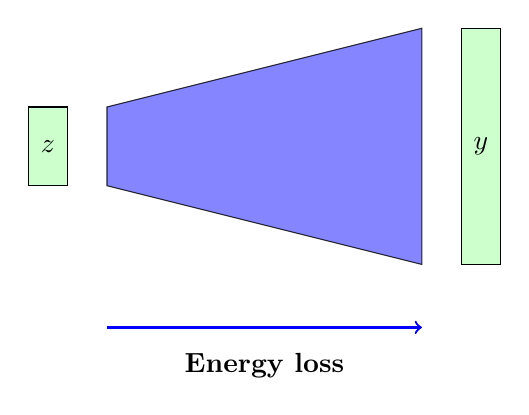
\begin{tikzpicture}
            % Modal coordinate (z)
            \draw[fill=green!20] (-3, 1) rectangle (-2.5,2);
            \node at (-2.75, 1.5) {$z$}; % Label inside the rectangle
            
            % Displacement (u)
            \draw[fill=green!20] (2.5,0) rectangle (3,3);
            \node at (2.75, 1.5) {$y$}; % Label inside the rectangle
            
            % Energy loss transition
            \draw[fill=blue!60,opacity=0.8] (-2,1) -- (2,-0) -- (2,3) -- (-2,2) -- cycle;
            \node[below] at (0,-1) {\textbf{Energy loss}};
            
            % Energy loss arrow
            \draw[thick,blue,->] (-2,-0.8) -- (2,-0.8);
        
        \end{tikzpicture}
\end{center}
    
\end{frame}

\begin{frame}
    \frametitle{Dynamic simulation - Twisting Beam}
    \begin{itemize}
        \item The beam is twisted by applying a gradual torque at the end.
        \item The main component of the simulation is the objective function that must be minimized.
        \item I tried to use 
        \[
              z_{n+1} = \underset{z}{\argmin}  \frac{1}{2h^2} \norm{n(z) - 2u_n + u_{n-1}}^2_M + E(n(z))
        \]
        but as we will see it behaves poorly.
    \end{itemize}
\end{frame}

\begin{frame}
    \frametitle{Dynamic simulation - Twisting Beam}
    \begin{center}
        \animategraphics[width=0.8\textwidth, autoplay, loop]{12}{Images/beam_linear/frames/frame}{0}{27}
    \end{center}
\end{frame}

\begin{frame}
    \frametitle{Dynamic simulation - Twisting Beam}
    \begin{itemize}
        \item By adding a term to keep the torque stable, the optimization problem behaves better.
        \item The term computes the virtual work and compares it to the expected torque (the one present in the simulation).
        \item The term is added minimizing the difference between the virtual work and the expected torque
        \[
            \begin{split}
                z_{n+1} = \underset{z}{\argmin}  \frac{1}{2h^2} \norm{n(z) - 2u_n + u_{n-1}}^2_M + E(n(z)) \\ + \norm{\tau - \tau_{\text{expected}}}^2
            \end{split}
        \]
    \end{itemize}
\end{frame}

\begin{frame}
    \frametitle{Animated Beam Deformation}
    \begin{center}
        \animategraphics[width=0.8\textwidth, autoplay, loop]{12}{Images/beam_deformation/frames/frame}{0}{43}
    \end{center}
\end{frame}


\begin{frame}
    \frametitle{Dynamic simulation - Gravity}
    \begin{itemize}
        \item The beam is immersed in a gravitational field.
        \item The objective function is the same as before, but the torque is replaced by the gravitational potential energy.
        \[
            \begin{split}
                z_{n+1} = \underset{z}{\argmin}  \frac{1}{2h^2} \norm{n(z) - 2u_n + u_{n-1}}^2_M + E(n(z)) \\ + \text{Potential Energy}
            \end{split}
        \]
        \item Also in this case the simulation is far from reality, but at least gravity is correctly captured.
    \end{itemize}
\end{frame}

\begin{frame}
    \frametitle{Animated Beam Deformation}
    \begin{center}
        \animategraphics[width=0.8\textwidth, autoplay, loop]{12}{Images/beam_gravity/frames/frame}{1}{84}
    \end{center}
\end{frame}


\begin{frame}
    \frametitle{Challenges \& Next Steps}
        \begin{itemize}
            \item \textbf{Two critical hurdles:}
                  \begin{itemize}
                    \item Network struggling to capture essential non-linearities in modes
                    \item Objective functions need meaningful physics-based tailoring
                  \end{itemize}
            \item \textbf{Seeking input:} Are there similar approaches worth exploring?
                  \begin{itemize}
                    \item Similar methods in the literature?
                    \item Maybe randomly sampling the latent space is not the best approach?
                    \item Better simulation techniques for validation
                  \end{itemize}
        \end{itemize}
\end{frame}

% Q&A
\begin{frame}
    \begin{center}
        \color{blue} \Huge{Questions?}
    \end{center}

\end{frame}
\end{document}

